\section{Eisengehalt}

\subsection{Arbeitsgrundlagen}

\subsection{Durchf\"{u}hrung}

\subsubsection*{Versuchsanordnung}


\subsubsection*{Messergebnisse}

\begin{center}
    \begin{threeparttable}
        \caption{Gemessene Gr\"ossen}
        \begin{tabular}{ccc}
            \toprule
            Messung & Eisengehalt (\%) & Absoluter Fehler (\%) \\
            \midrule
            1   & 20.3  & 1.2 \\
            2   & 21.9  & 1.3 \\
            3   & 21.1  & 1.1 \\
            4   & 19.6  & 0.8 \\
            5   & 19.9  & 1.3 \\
            6   & 18.0  & 1.3 \\
            7   & 19.4  & 1.0 \\
            8   & 22.2  & 2.0 \\
            9   & 21.6  & 0.8 \\
            \bottomrule
        \end{tabular}
        \begin{tablenotes}
            \small
            \item \textbf{Hinweis:} Daten wurde vom Auftragsdokument kopiert.
        \end{tablenotes}
    \end{threeparttable}
\end{center}

Der einfache Mittelwert berechnet sich mit der Formel
\[ \bar{x}_{einfach} = \frac{1}{9} \sum_{i=1}^{9} x_i = \underline{\underline{20.4 \textrm{\%}}} \]
wobei $x_i$ das Eisengehalt in Prozent ist.

Der gewichtete Mittelwert l\"asst sich mit der Formel
\[ \bar{x}_{gewichtet} = \frac{ \sum_{i=1}^{9} g_{\bar{x}_i} \cdot x_i}{ \sum_{i=1}^{9} g_{\bar{x}_i}} = \underline{\underline{20.4 \textrm{\%}}} \]
berechnen, wobei
\[ g_{\bar{x}_i} = \frac{1}{s_{\bar{x}_i}^2} \]
und $x_i$ der Eisengehalt in Prozent ist und $g_{\bar{x}_i}$ der absoluter Fehler in Prozent ist.

Der einfache Fehler berechnet sich mit der Formel
\[ s_{\bar{x}_{einfach}} = \sqrt{ \frac{ \sum_{i=1}^{9} (x_i - s_{\bar{x}})^2}{ 9 \cdot (9-1) }} = \underline{\underline{0.5 \textrm{\%}}} \]
wobei $x_i$ der Eisengehalt in Prozent ist und $s_{\bar{x}}$ der \emph{einfache} Mittelwert ist.

Der gewichtete Fehler berechnet sich mit der Formel
\[ s_{\bar{x}_{gewichtet}} = \frac{1}{ \sqrt{ \sum_{i=1}^{9} g_{\bar{x}_i} } } = \underline{\underline{0.4 \textrm{\%}}}  \]


\subsubsection*{QtiPlot}

\begin{figure}[H]
    \center
    \caption{XY-Scatter der gemessenen Eisengehalte mit Fehler}
    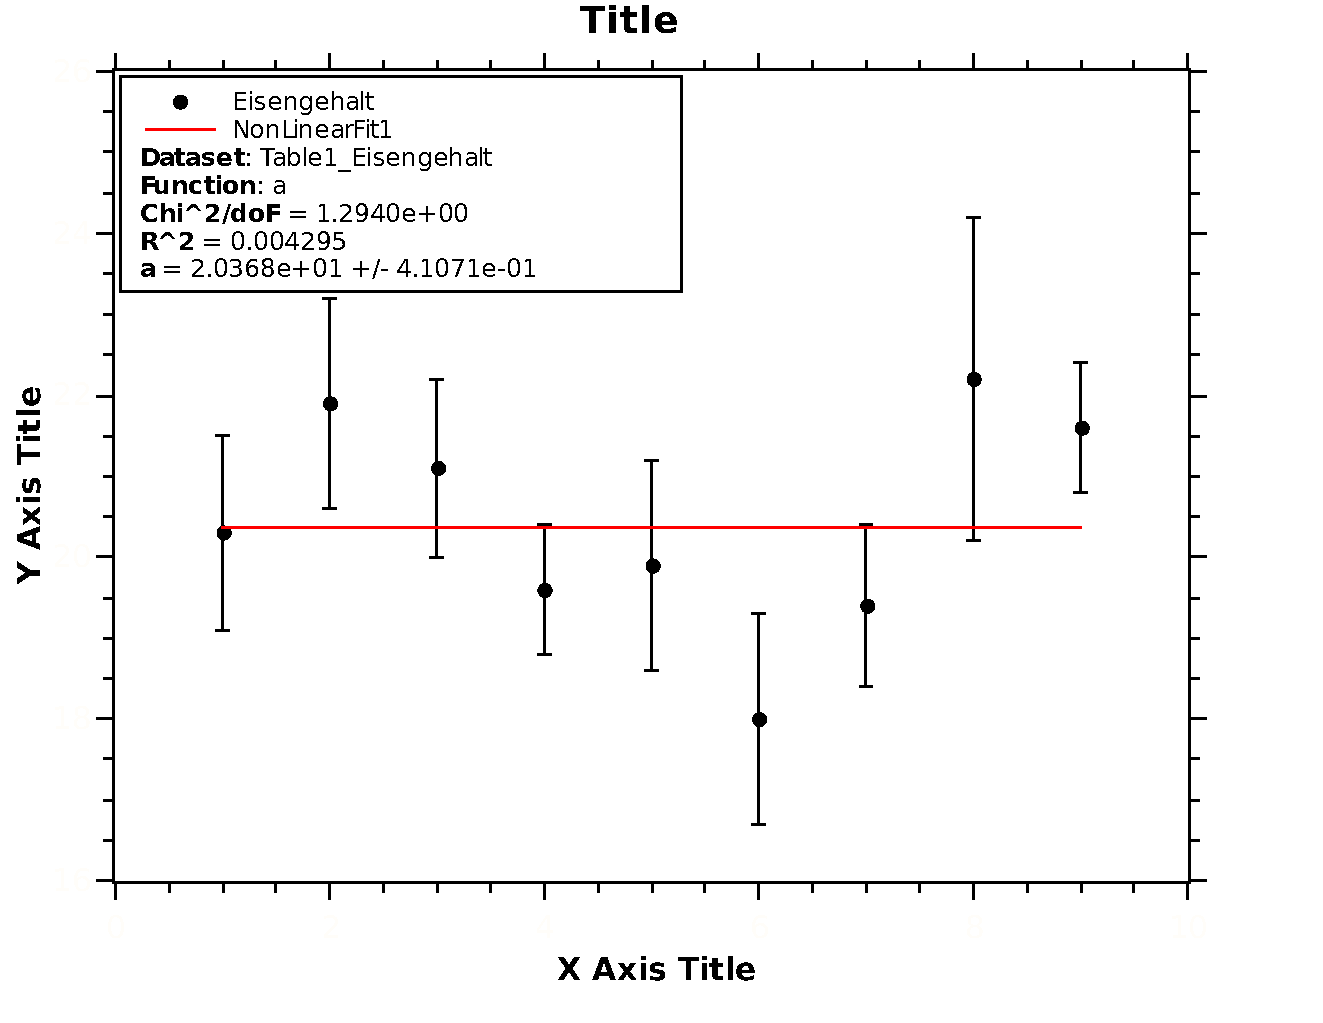
\includegraphics[width=.85\textwidth]{qtiplot/eisengehalt}
    \label{fig:eisengehalt}
\end{figure}

